\chapter{Punktesortierung in Schachbrettmustern}
\label{sec:schachbrettAlg} 


Für die reelle Rekonstruktion, wie sie in Kapitel \ref{sec:real} beschrieben wird, sind die korrespondierenden Punkte


In diesem Teil der Masterthesis soll am Ende ein Algorithmus entstehen, welcher durch einen bereits bestehenden Algorithmus zur Detektion von Eckpunkten eines Schachbretts, eine Liste an Eckpunkten bekommt und diese auf deren Nachbarschaftsverhältnisse prüft. Die Schachbretter können dabei sowohl Kissen- als auch Tonnennverzeichnungen aufweisen und oder perspektivisch verzerrt sein. Mit den Algorithmus sollen Punkte wissen in welchen Reihen sie sich sowohl in x- als auch y-Richtung befinden. Jeder Punkt bekommt also eine Indexnummer in x-, sowie y-Richtung beziehungsweise in unserem Beispiel wird die y-Koordinate als \textit{j} bezeichnet und die x-Koordinate als \textit{i}, zugewiesen. Jeder Punkt bekommt mit Hilfe von den Mathematica eigenen \textit{Associations} einen \textit{Key} mit \textit{NeighbourJ} und \textit{NeighbourI} zugeteilt. Mit Hilfe dieser \textit{Keys} kann dann später bei einem Stereobildpaar zum Beispiel die Korrespondierenden Eckpunkte der Schachbretter rausgesucht werden, was vielleicht genauere Ergebnisse liefert also die Suche von Hand. Des weiteren kann dieser Algorithmus in späteren Projekten vielleicht bei der Rausrechnung von Verzeichnungen hilfreich sein.\\

%Irgendwie noch definieren das x = i und y = j sein sollen. 
%Bsp:
%Für die Sortierung der Schachbrettpunkte, wird das Schachbrett in ein Koordinatensystem, mit vertikaler Achse $i$ und horizontaler Achse $j$, gelegt.

\section{Sortierungsalgorithmus}

Für die Sortierung der Schachbrettpunkte, wird das Schachbrett in ein Koordinatensystem, mit vertikaler Achse $i$ und horizontaler Achse $j$, gelegt. Um das Schachbrett herum wird ein Rahmen definiert. Die Punkte mit der maximale $i$-Koordinate und der minimalen $i$-Koordinate Begrenzen die oberen und unteren Kanten des Rahmens. Die Punkte mit der minimalen $j$-Koordinate und der Punkt mit der  maximalen $j$-Koordinate Begrenzen die vertikalen Kanten des Rahmens. In Abbildung \ref{fig:7.1} sind die roten Begrenzungskanten um das Schachbrett zu sehen.\\

Der durch den Rahmen begrenzte Bereich wird in gleich viele Reihen wie Spalten unterteilt, so dass eine Gitter entsteht. Die so entstehenden Zellen des Gitters werden in $i$-Richtung sowie in $j$-Richtung durchgezählt und bekommen somit jeweils zwei Indizes $(i_i,j_i)$, welche sie eindeutig identifizieren.\\

In den angelegten $ConstantArrays$ namens $JSplits$ und $ISplits$ werden die Begrenzungen Zellen in $i$- und $j$-Richtung gespeichert. Die Begrenzungen der Zellen werden über die Distanz des Punktes mit der minimalen $j$-Koordinate zum Punkt mit der maximalen $j$-Koordinate geteilt durch die gewünschte Anzahl der Zellen, definiert. Selbiges gilt für die Unterteilung der Zellen in $i$-Richtung. \\ 

Alle Punkte in den Zellen mit den Indizes $i=1$ und $j \leq  j_{max}$ werden als mögliche Startpunkte gekennzeichnet. In Abbildung \ref{fig:7.1} befinden sich die möglichen Startpunkte innerhalb des blauen Bereichs. Die Suche nach einem Startpunkt und auch nach den ersten Punkten in zwei Richtungen vom Startpunkt aus, ist relativ komplex. Der Grund hierfür ist, dass sämtliche Schachbretter wie in \ref{sec:SchachAlgBeispiele} gezeigt, in Betracht gezogen werden müssen. Um Anhand des Algorithmus später korrespondierende Punkte in zwei Aufnahmen des Schachbretts finden kann, sollte gewährleistet sein, dass der Startpunkt immer an der selben Ecke eines Schachbretts platziert wird.\\

Innerhalb der blau gefärbten Fläche wird nach einem Startpunkt gesucht. Die Suche nach einem Startpunkt wird pro $i$- und $j$-Richtung in zwei Abfragen unterteilt.\\

In der ersten Abfrage für die $i$-Richtung, wird innerhalb der ersten Zellenreihe entlang der $j$-Koordinatenachse nach dem Punkt mit der kleinsten $i$-Koordinate gesucht.Dieser Punkt wird als möglicher erster Startpunkte in der Variablen $VecI$ gespeichert.\\

Danach wird geprüft ob es innerhalb der ersten Zellen in $i$-Richtung einen weiteren Punkt gibt dessen $j$-Koordinate kleiner ist als die des momentan gesetzten Punktes $VecI$, wird ein solcher Punkt gefunden, so wird dieser Punkt als neuer $VecI$ gesetzt, sofern seine $i$-Koordinate nicht größer ist als die des zuvorigen $VecI$ plus einem Pufferwert. Durch den Puffer wird verhindert, dass ein Punkt als $VecI$ gesetzt wird, welcher sich möglicherweise schon in der zweiten Reihe der Schachbrettpunkte befinden würde. In Abbildung \ref{fig:7.1} ist $VecI$ mit als oranger Punkt abgebildet.\\

%\begin{figure}[!htb]
%	\minipage{0.48\textwidth}
%	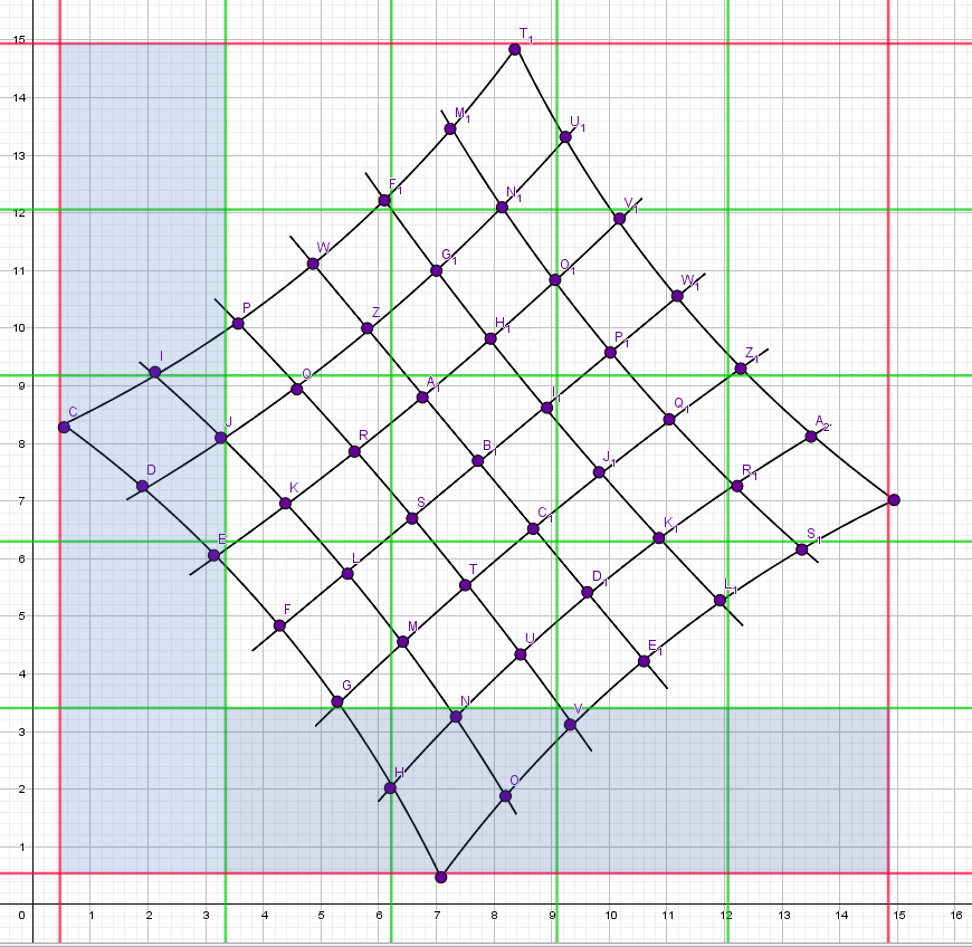
\includegraphics[width=\linewidth]{images/VerzeichnetesSchachbrett_0.png}
%	\caption{ }
%	\label{fig:7.1}
%\end{figure}
%	\endminipage\hfill
\begin{figure}[!htb]
	\centering
	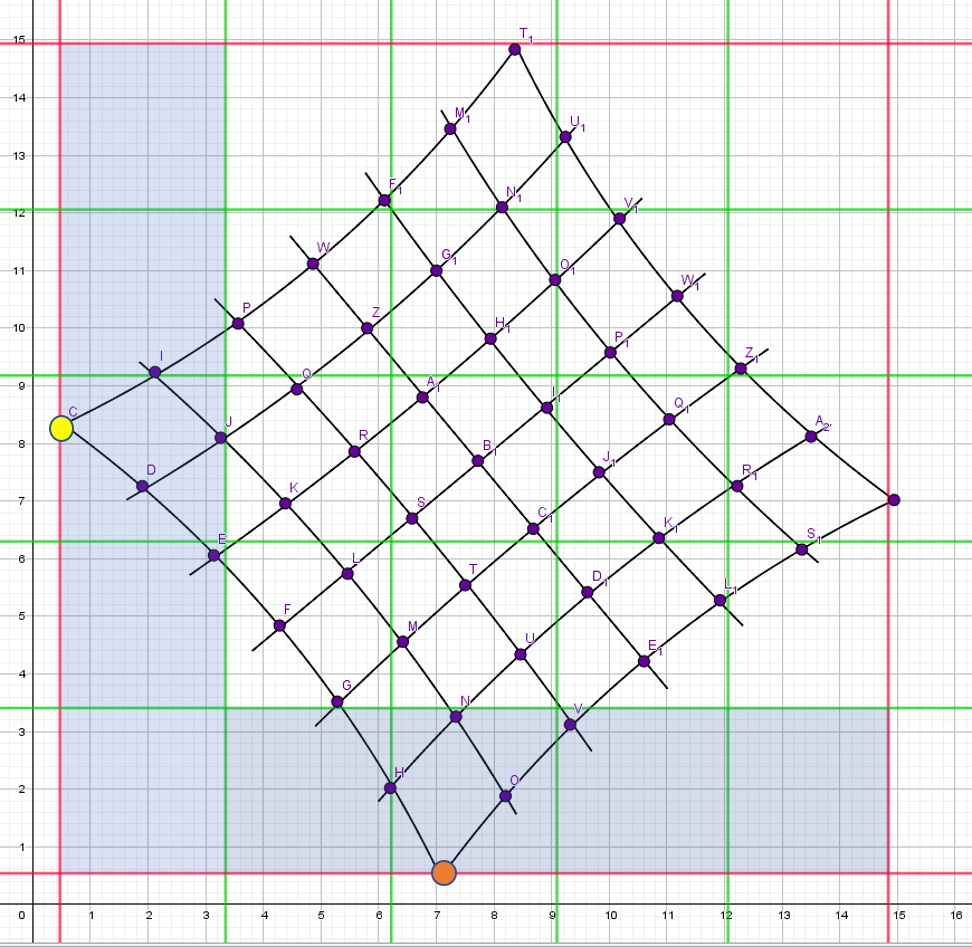
\includegraphics[width=0.8\linewidth]{images/VerzeichnetesSchachbrett_1.png}
	\caption[Startpunktsuche in Schachbrettpunkten]{Die in blau markierten Bereiche beinhalten die möglichen Startpunkte. Der Bereich entlang der horizontalen $j$- Achse bildet die erste Suchfensterreihe in $i$-Richtung. Der blaue Bereich entlang der vertikalen $i$-Achse bildet die erste Suchfensterreihe in $j$-Richtung. Der gelbe Punkt steht für den Punkt welcher als $VecJ$ bezeichnet wurde und der orange Punkt ist derjenige Punkt, welcher als $VecI$ bestimmt wurde}
	\label{fig:7.1}
\end{figure}


Für die erste Abfrage in $j$-Richtung, werden die Zellen entlang der vertikalen $i$-Koordinatenachse mit den Indizes $j=1$ und $i \leq i_max$, nach dem Punkt gesucht, welcher die geringste $j$-Koordinate besitzt. Dieser Punkt wird als voläufiges $VecJ$ bestimmt.\\

Danach wird auch hier geprüft, ob es innerhalb der ersten Suchfensterreihe in $j$-Richtung einen weiteren Punkt gibt, dessen $i$-Koordinate kleiner ist als die des momentan gesetzten Punktes $VecJ$. Trifft des Weiteren zu, dass die $j$-Koordinaten des neu gefundenen Punktes kleiner ist als die $j$-Koordinate plus einem Pufferwert des momentanen $VecJ$ , so wird dieser als neuer Punkt als $VecJ$ festgelegt. In Abbildung \ref{fig:7.1} ist $VecJ$ als gelber Punkt zu sehen.\\

Je nachdem wie das Schachbrett liegt oder welche Verzerrungen es aufweist, kann es sein dass $VecI$ und $VecJ$ den selben Punkt ergeben haben, was den Startpunkt $StartPoint$ eindeutig identifiziert, wie es in Beispiel \ref{PerspVerzerrt} oder auch \ref{KissenVerz} der Fall war. Andererseits kann es auch wie in Abbildung \ref{fig:7.1} zu sehen ist sein, dass $VecI$ und $VecJ$ sich unterscheiden. In solchen Fällen wurde beschlossen das $VecJ$ als Startpunkt festgelegt wird. $Startpoint$ bekommt eine Association \cite{Mathematica}, welche insgesamt sechs sogenannte Keys speichert. Die $Association$ beinhaltet sowohl die Keys $CoordJ$ und $CoordI$, welche die jeweiligen $i$- und $j$- Koordinaten des Punktes speichern. Daneben gibt es noch die beiden Keys $CellI$ und $CellJ$, welche die Information speichern in welcher Zelle sich der Startpunkt befindet und letztendlich gibt es noch die Keys $NeighbourI$ und $NeighbourJ$, welche die Information speichern, der wievielte Punkt der Startpunkt in $i$- und $j$-Richtung ist. Im Falle des Startpunktes wird fest gelegt, dass er sowohl in $i$- als auch in $j$-Richtung der erset Punkt ist und somit die gilt $NeighbourI = 1$ und $NeighbourJ = 1$\\

Diese Informationen werden für jeden weiteren sortierten Punkt in einer $Association$ verwaltet. Diese $Associations$ werden wiederum in zwei Listen gespeichert. In die Liste $CheckPoints$ werden von einem Punkt nur die Key $CoordI$ und $CoordJ$ gespeichert. Anhand der $Checklist$ kann überprüft werden, ob ein Punkt bereits sortiert wurde.  Die Liste $SortedPoints$ beinhaltet alle Informationen über die Punkte.  

(HIER WEITER SCHREIBEN!!)

Nachdem ein Startpunkt bestimmt ist, werden nun die ersten beiden Punkte in $i$-und $j$-Richtung bestimmt. Diese Punkte werden später in die Variablen $NextI$ und $NextJ$ gespeichert.








\begin{figure}[!htb]
	\minipage{0.48\textwidth}
	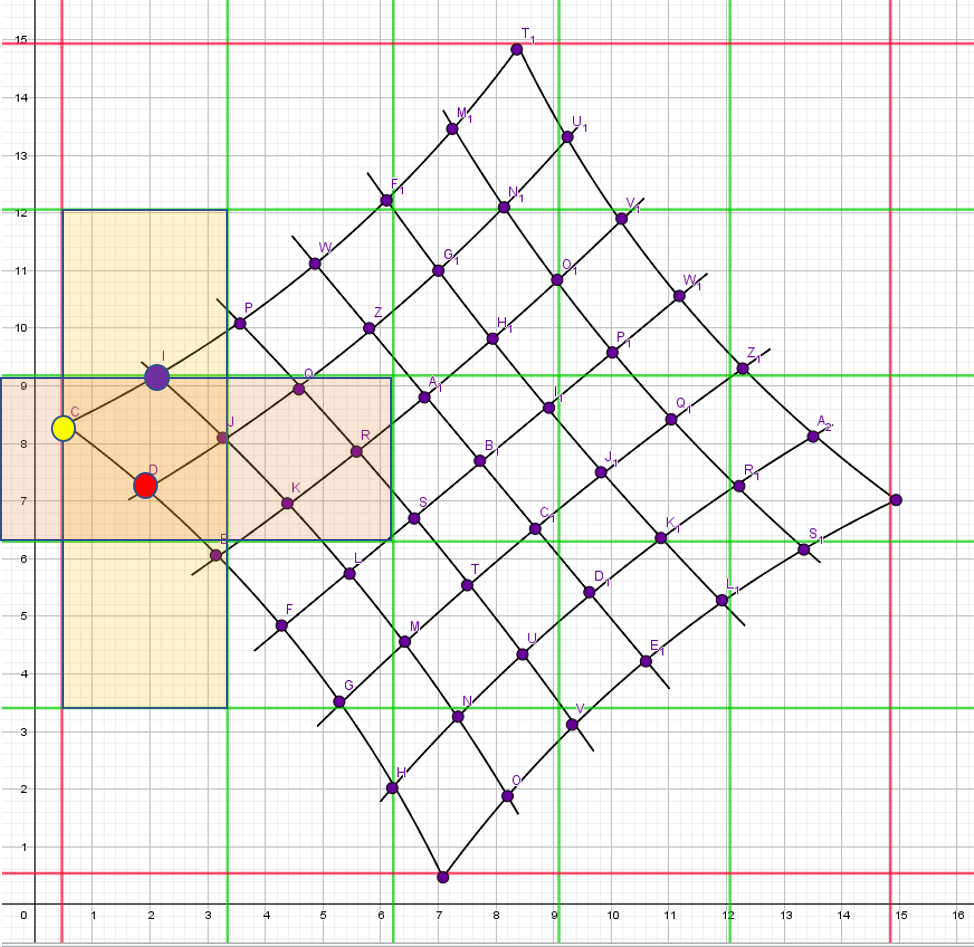
\includegraphics[width=\linewidth]{images/VerzeichnetesSchachbrett_2.png}
	\caption{}
	\label{fig:awesome_image1}
	\endminipage\hfill
	\minipage{0.48\textwidth}
	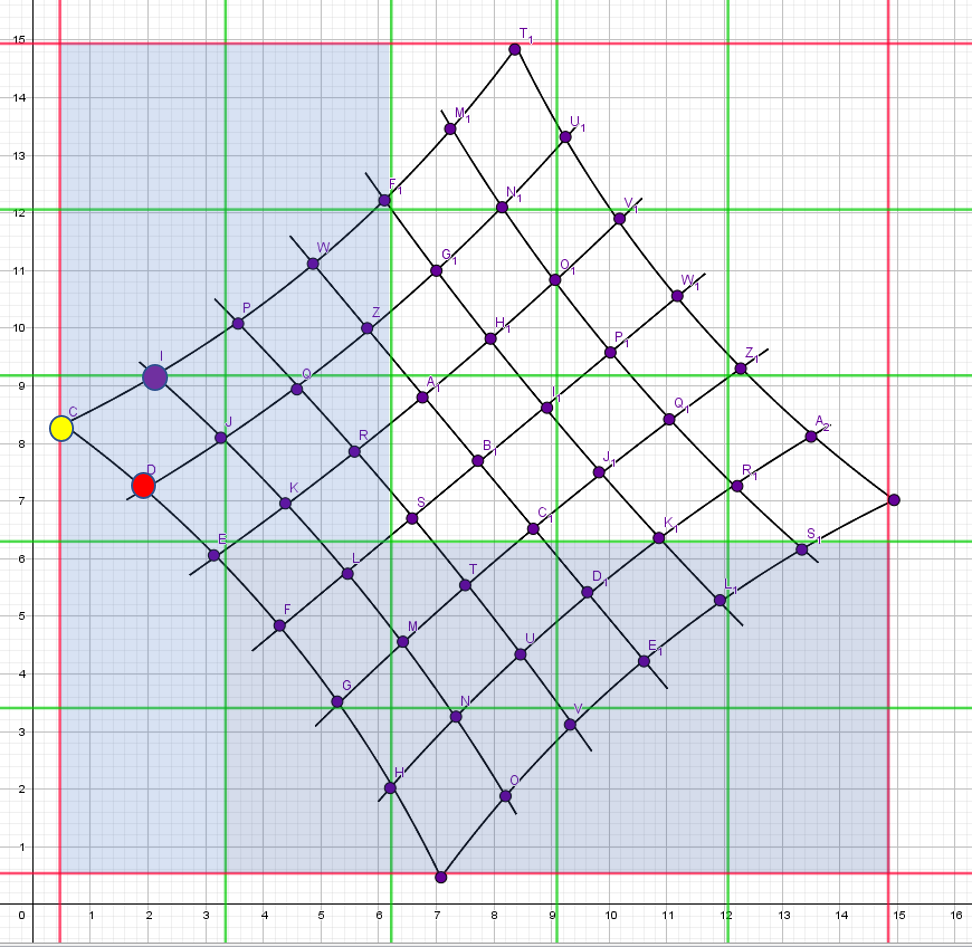
\includegraphics[width=\linewidth]{images/VerzeichnetesSchachbrett_3.png}
	\caption{}
	\label{fig:awesome_image2}
	\endminipage\hfill
	%	\caption{Die mit dem \textit{SURF}-Algorithmus gefundenen Punkte sind mit den gelben Ziffern im Bild gekennzeichnet}
\end{figure}

\begin{minipage}{\linewidth}
	\centering
	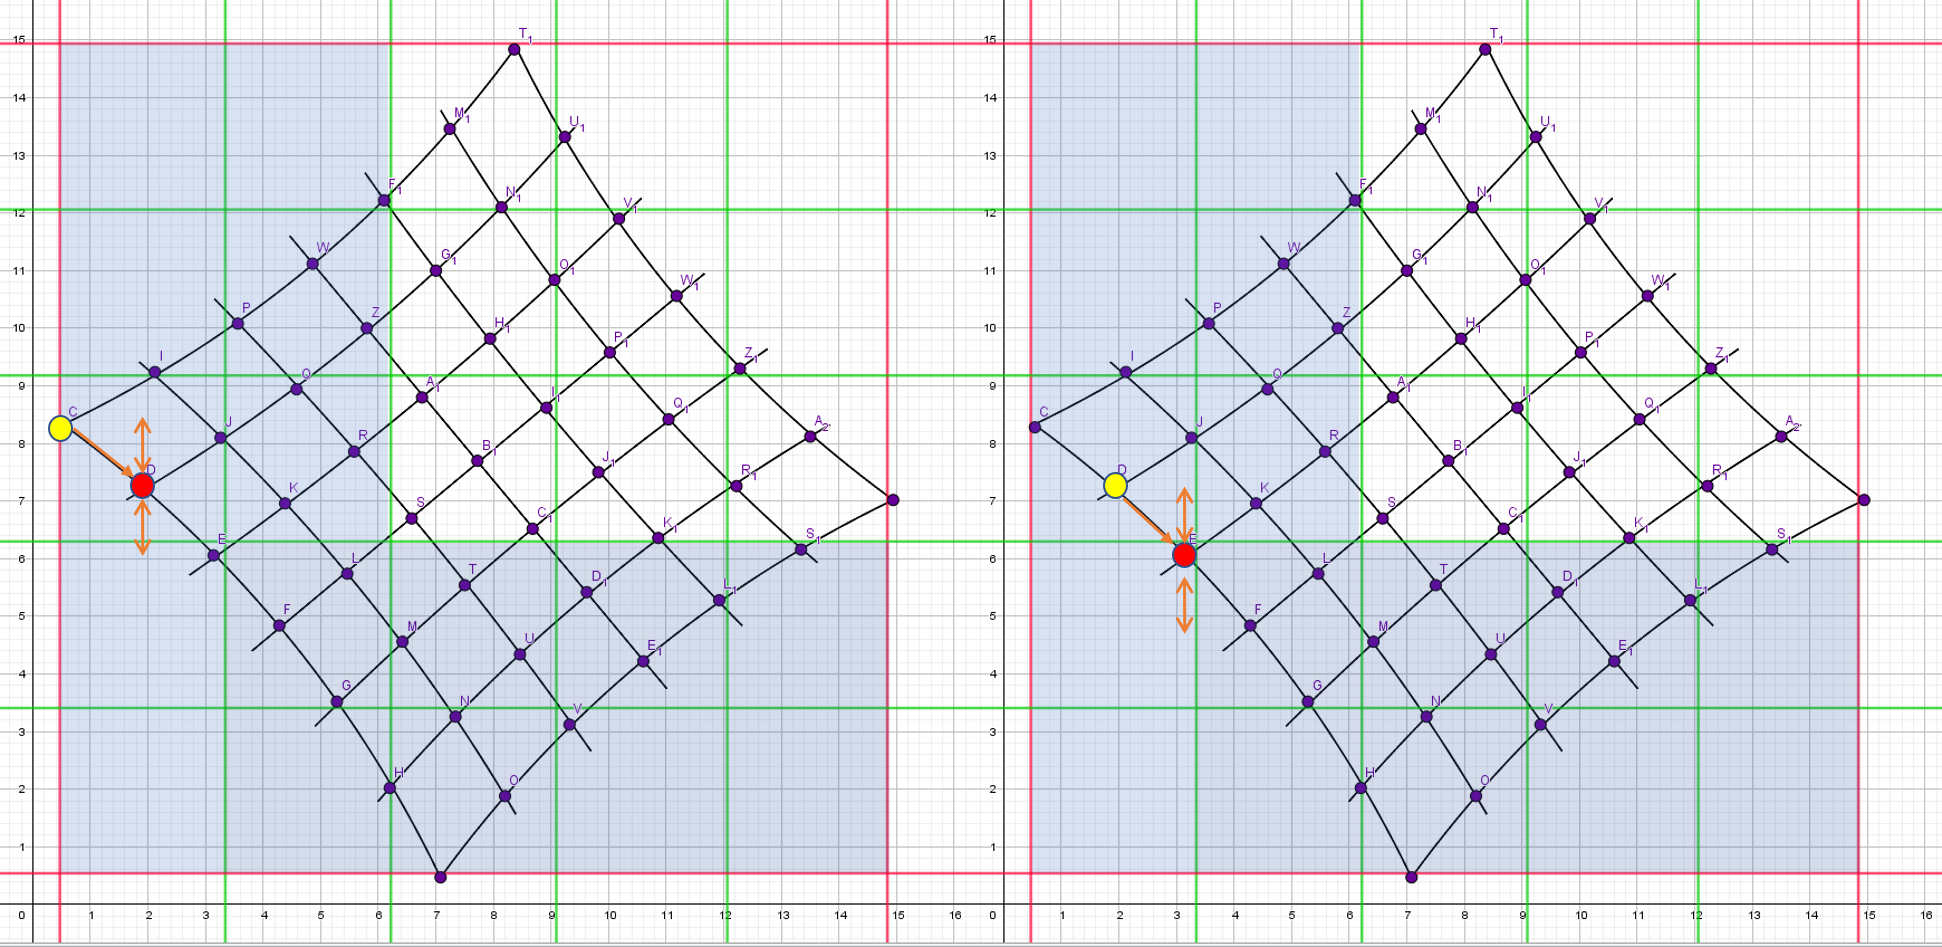
\includegraphics[width=1\linewidth]{images/VerzeichnetesSchachbrett_4.png}
	\captionof{figure}{Klassendiagramm}
\end{minipage}\\

\begin{minipage}{\linewidth}
	\centering
	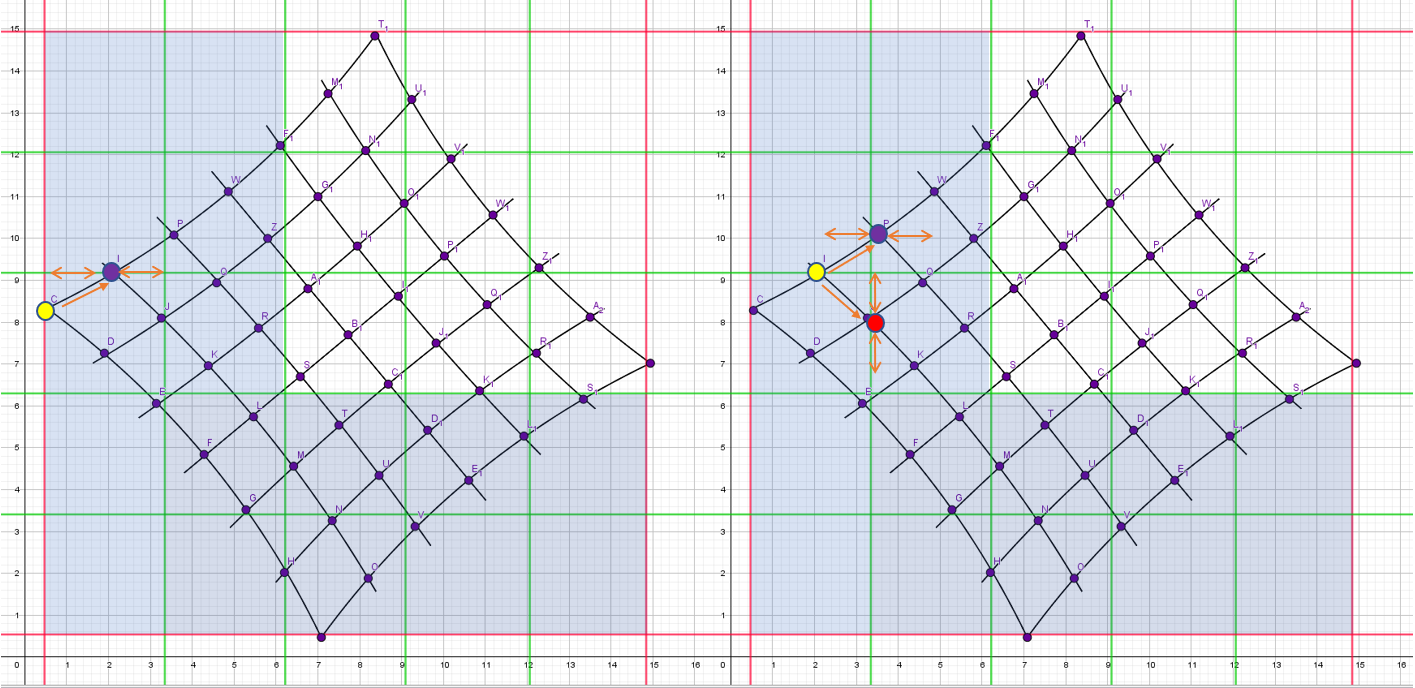
\includegraphics[width=1\linewidth]{images/VerzeichnetesSchachbrett_5.png}
	\captionof{figure}{Klassendiagramm}
\end{minipage}\\

\begin{minipage}{\linewidth}
	\centering
	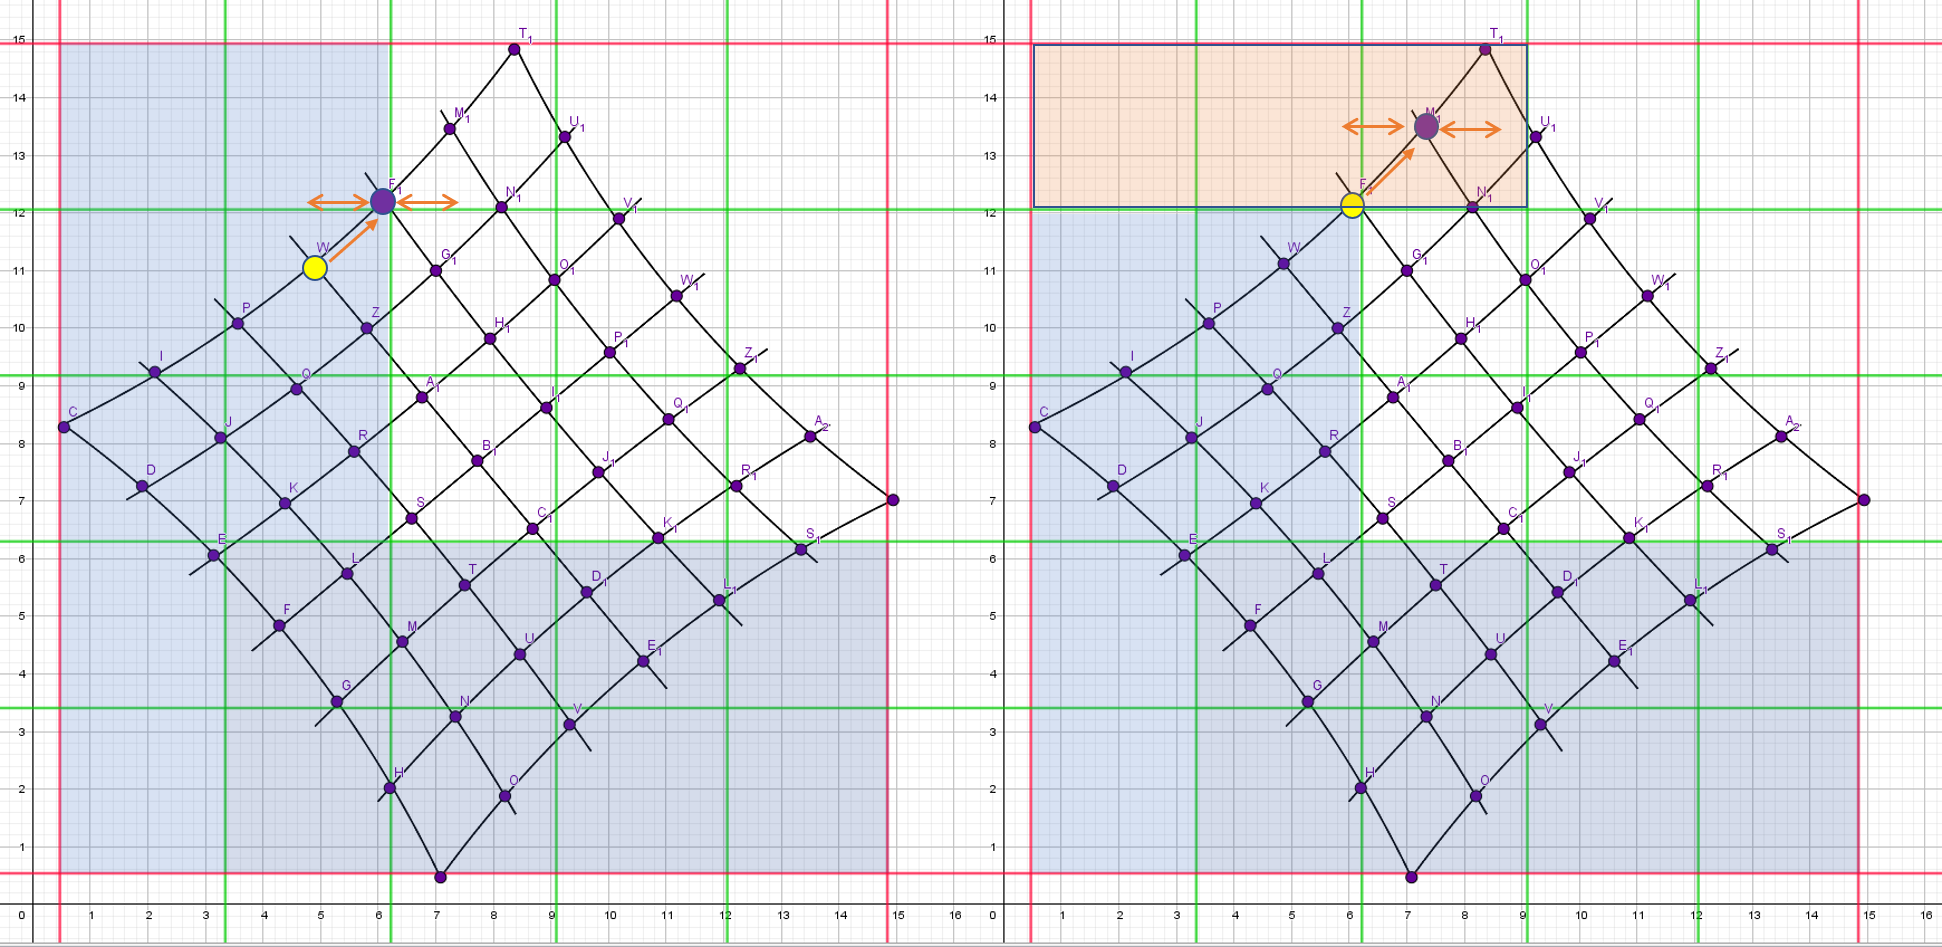
\includegraphics[width=1\linewidth]{images/VerzeichnetesSchachbrett_6.png}
	\captionof{figure}{Klassendiagramm}
\end{minipage}\\


\section{Extrembeispiele}
\label{sec:SchachAlgBeispiele}

In den folgenden Beispielen sieht man jeweils das Originalbild und ein Bild welches die durch den Algorithmus sortierten Punkte farbig ausgibt. Die grünen eingefärbten Punkte sind in den Bildern des Algorithmus die Nachbarn, welche sich in i-Richtung an der dritten Stelle befinden. Natürlich können auch andere Reihen oder auch einzelne Punkte abgefragt werden. 
\pagebreak

\begin{figure}[!htb]
	\minipage{0.48\textwidth}
	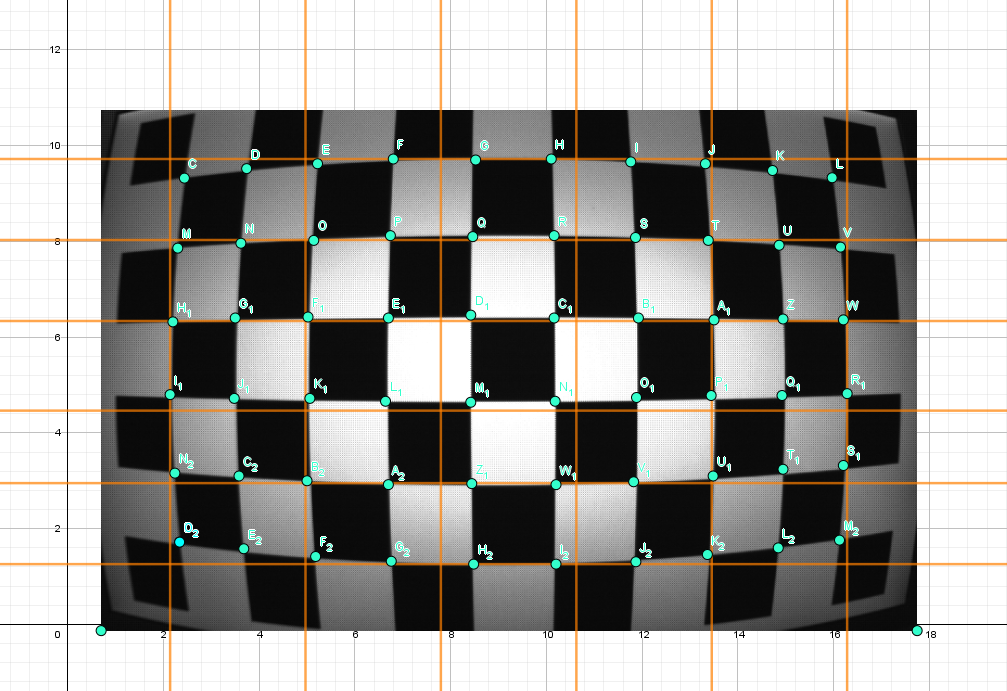
\includegraphics[width=\linewidth]{images/Tonnenverzeichnung.png}
	\caption{Bild eines Tonnenförmig verzeichneten Schachbretts}
	\label{fig:awesome_image1}
	\endminipage\hfill
	\minipage{0.48\textwidth}
	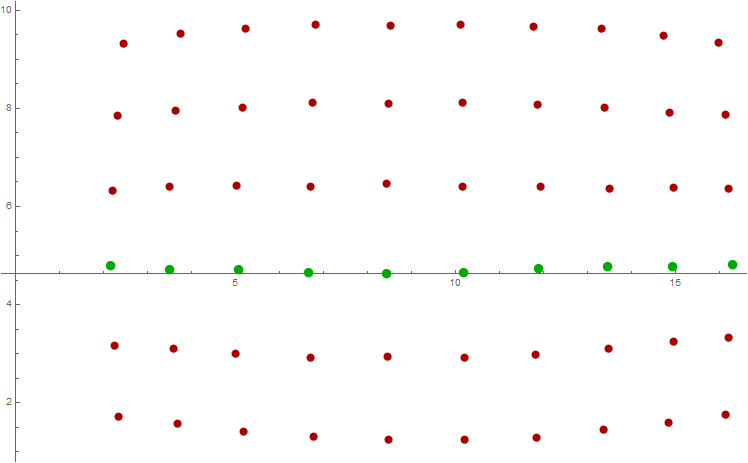
\includegraphics[width=\linewidth]{images/AlgTonnenverzeichnung.png}
	\caption{Algorithmisch detektierte Linie der dritten i-Reihe}
	\label{fig:awesome_image2}
	\endminipage\hfill
\end{figure}

\begin{figure}[!htb]
	\minipage{0.48\textwidth}
	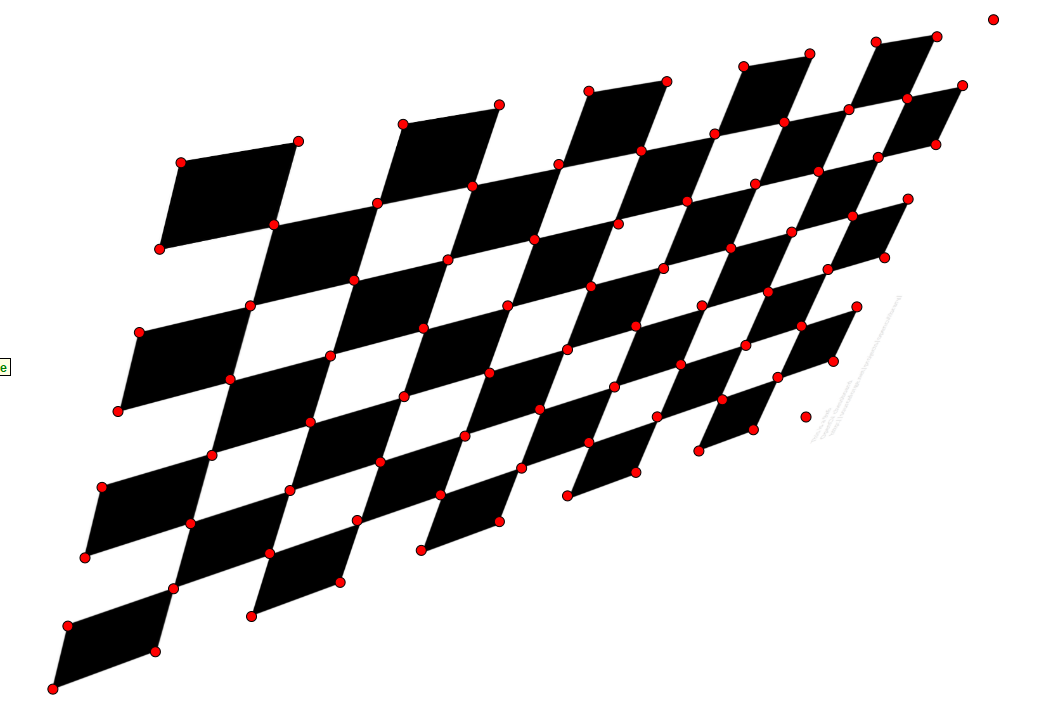
\includegraphics[width=\linewidth]{images/perspektivisch.png}
	\caption{Bild eines perspektivisch verzerrtem Schachbretts}
	\label{fig:awesome_image1}
	\endminipage\hfill
	\minipage{0.48\textwidth}
	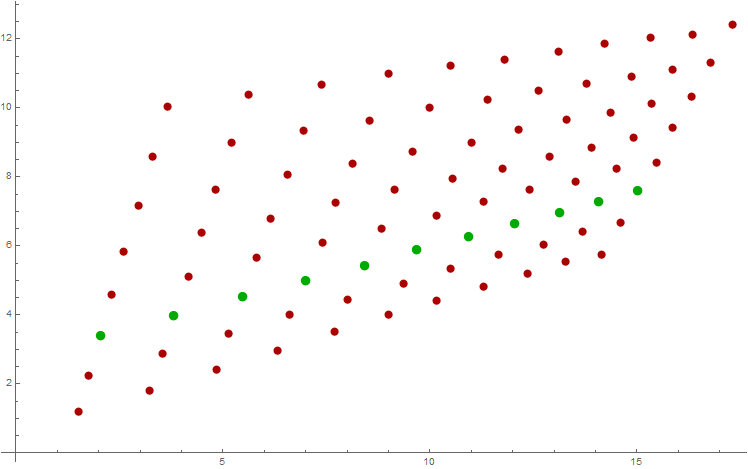
\includegraphics[width=\linewidth]{images/AlgPerspektifisch.png}
	\caption{Algorithmisch detektierte Linie der dritten i-Reihe}
	\label{fig:awesome_image2}
	\endminipage\hfill
\end{figure}


\begin{figure}[!htb]
	\minipage{0.48\textwidth}
	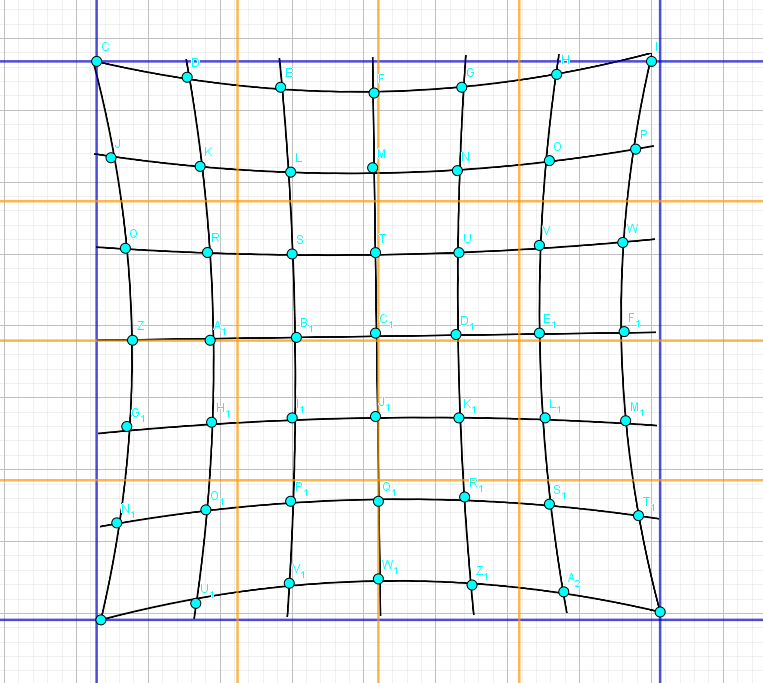
\includegraphics[width=\linewidth]{images/KissenVerzeichnung.png}
	\caption{Bild eines Kissenförmig verzeichnetem Schachbretts}
	\label{fig:awesome_image1}
	\endminipage\hfill
	\minipage{0.48\textwidth}
	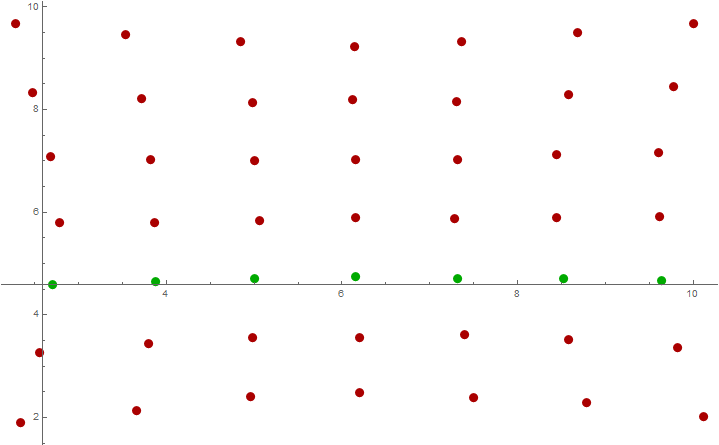
\includegraphics[width=\linewidth]{images/AlgKissen.png}
	\caption{Algorithmisch detektierte Linie der dritten i-Reihe}
	\label{fig:awesome_image2}
	\endminipage\hfill
\end{figure}

\begin{figure}[!htb]
	\minipage{0.48\textwidth}
	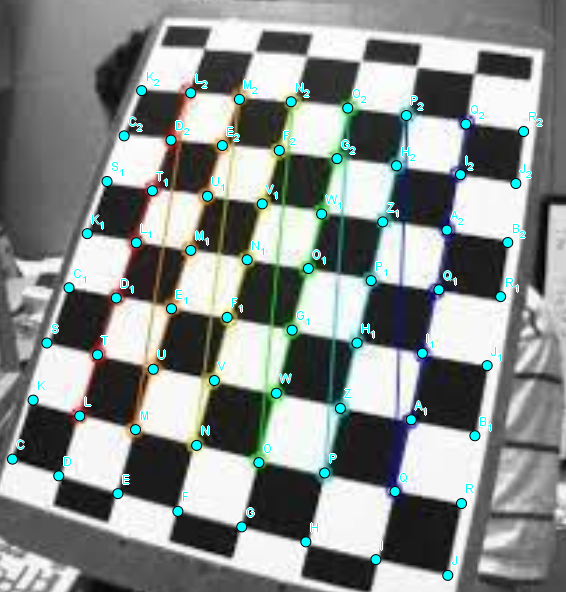
\includegraphics[width=\linewidth]{images/TonnePers.png}
	\caption{Bild eines Tonnenförmig verzeichnetem leicht perspektivisch verzerrtem Schachbretts(GRFIK AUSTAUSCHEN BILD IS KACKE)}
	\label{fig:awesome_image1}
	\endminipage\hfill
	\minipage{0.48\textwidth}
	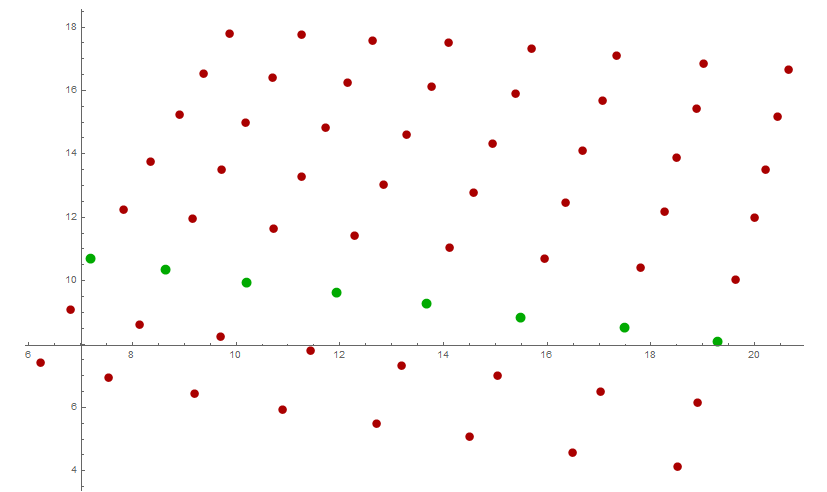
\includegraphics[width=\linewidth]{images/AlgTonnePers.png}
	\caption{Algorithmisch detektierte Linie der dritten i-Reihe}
	\label{fig:awesome_image2}
	\endminipage\hfill
\end{figure}

\begin{figure}[!htb]
	\minipage{0.48\textwidth}
	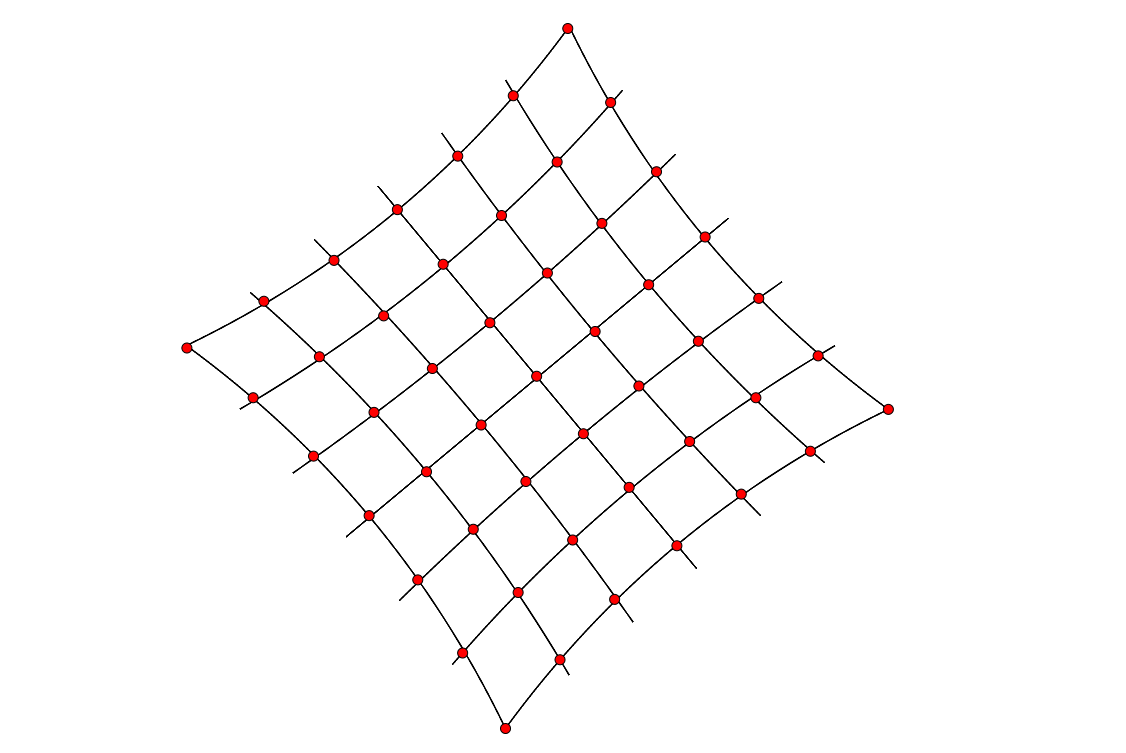
\includegraphics[width=\linewidth]{images/extrBsp.png}
	\caption{Bild eines Tonnenförmig verzeichnetem leicht perspektivisch verzerrtem Schachbretts}
	\label{fig:awesome_image1}
	\endminipage\hfill
	\minipage{0.48\textwidth}
	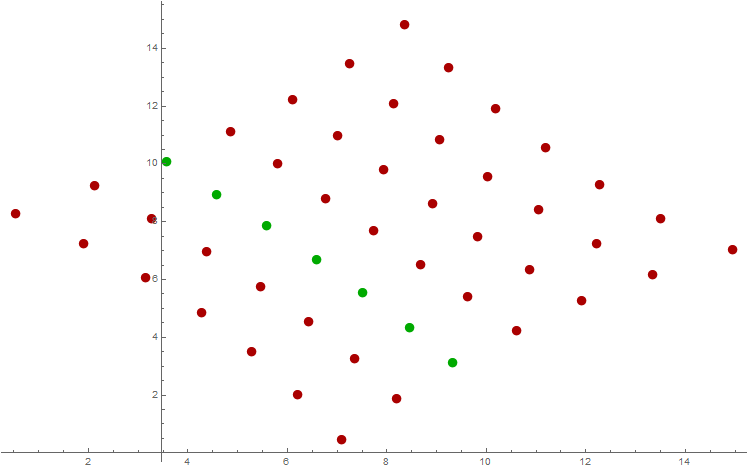
\includegraphics[width=\linewidth]{images/AlgExtrBsp.png}
	\caption{Algorithmisch detektierte Linie der dritten i-Reihe}
	\label{fig:awesome_image2}
	\endminipage\hfill
\end{figure}


\section{Modulübersicht}


\begin{minipage}{\linewidth}
	\centering
	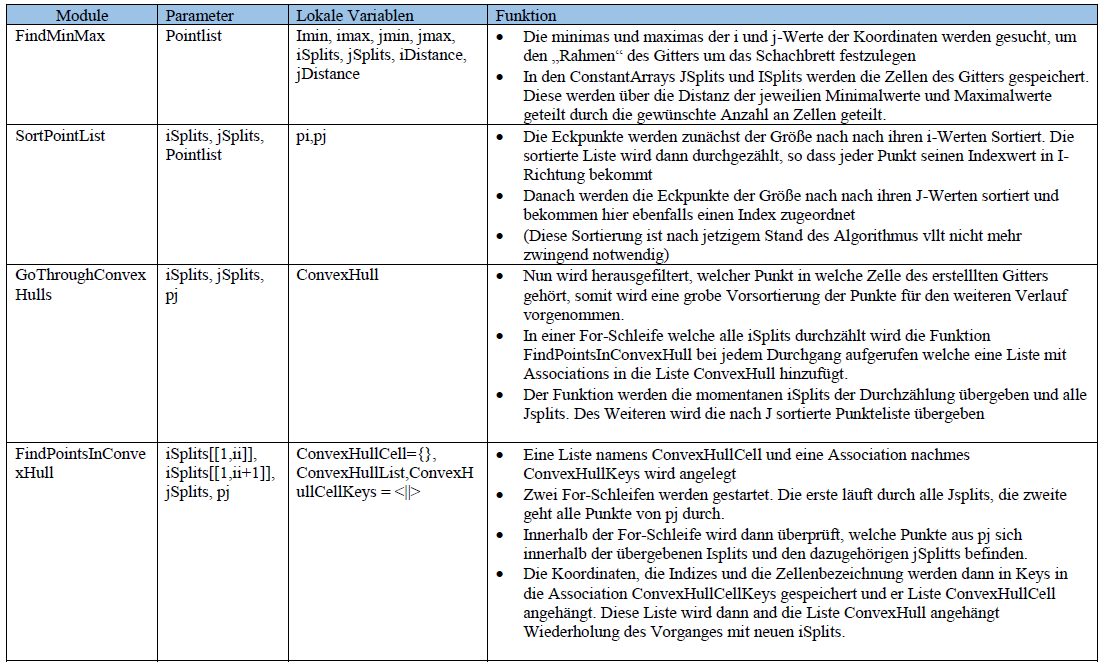
\includegraphics[width=1\linewidth]{images/KD1.png}
	\captionof{figure}{Klassendiagramm}
\end{minipage}
\begin{minipage}{\linewidth}
	\centering
	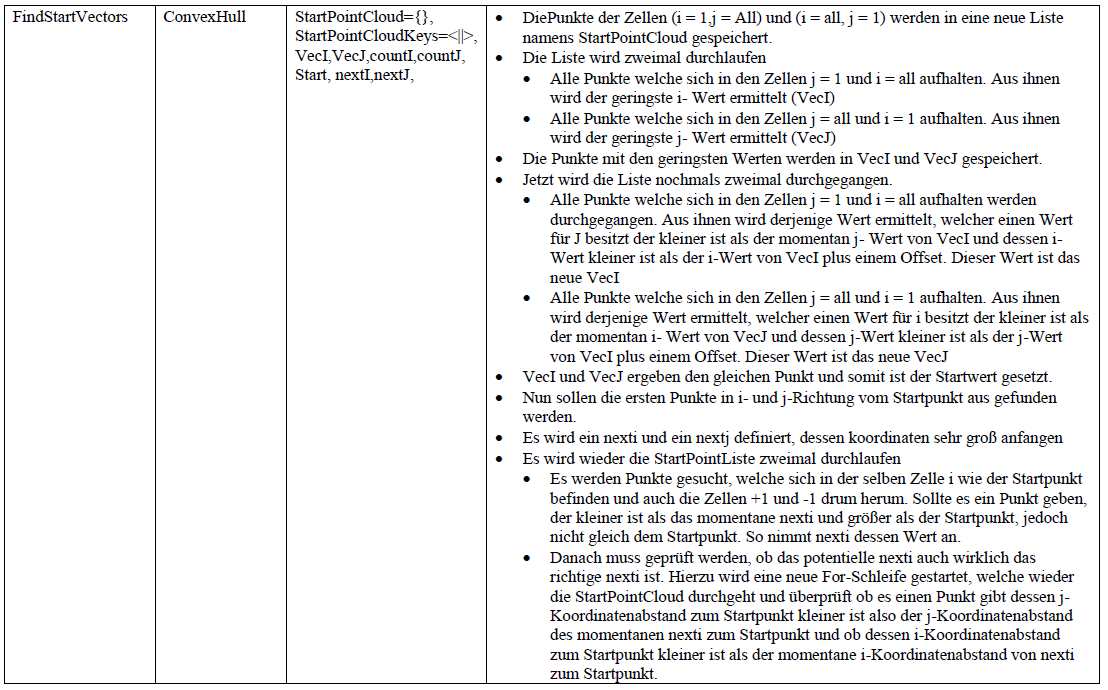
\includegraphics[width=1\linewidth]{images/KD2.png}
	\captionof{figure}{Klassendiagramm}
\end{minipage}
\begin{minipage}{\linewidth}
	\centering
	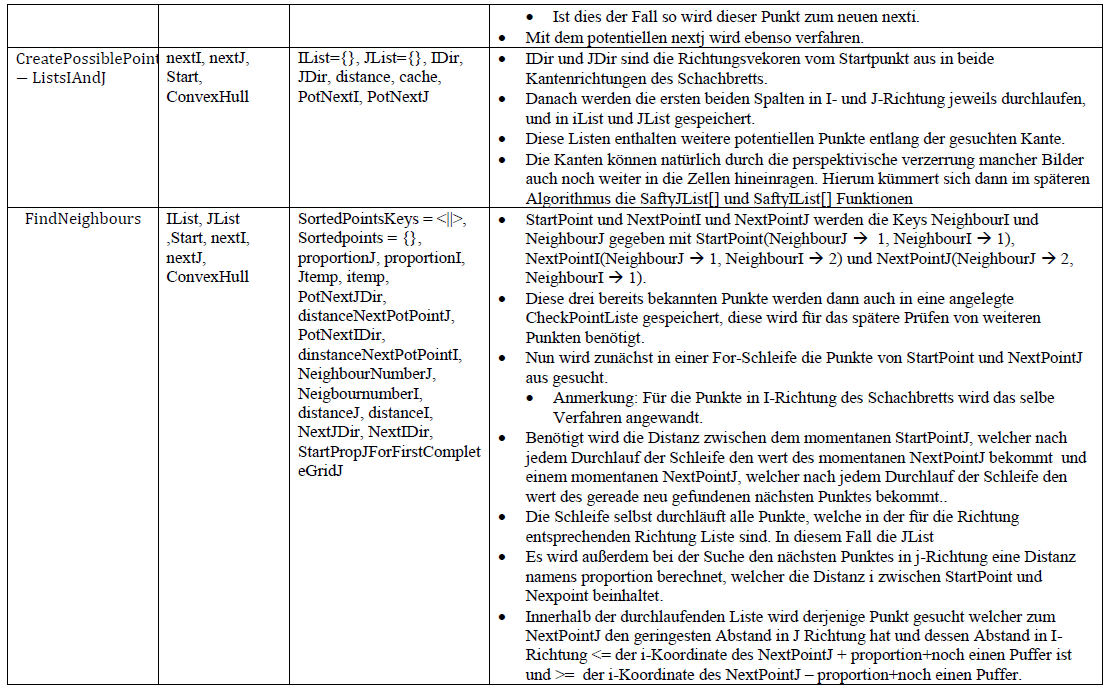
\includegraphics[width=1\linewidth]{images/KD3.png}
	\captionof{figure}{Klassendiagramm}
\end{minipage}
\begin{minipage}{\linewidth}
	\centering
	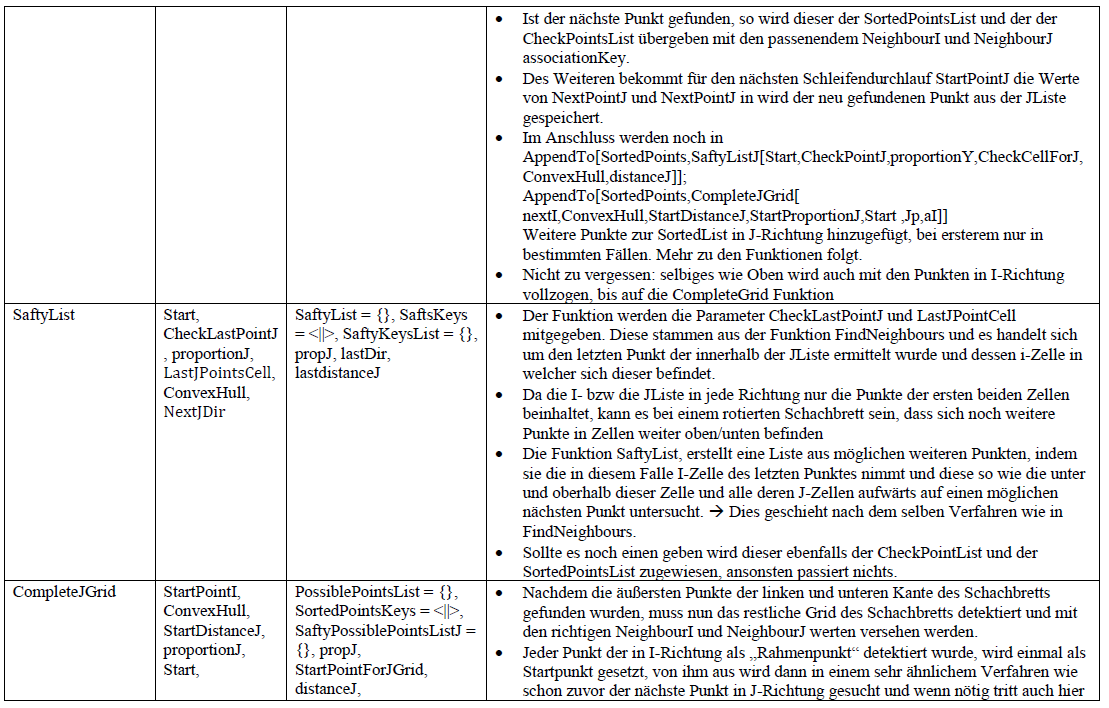
\includegraphics[width=1\linewidth]{images/KD4.png}
	\captionof{figure}{Klassendiagramm}
\end{minipage}
\begin{minipage}{\linewidth}
	\centering
	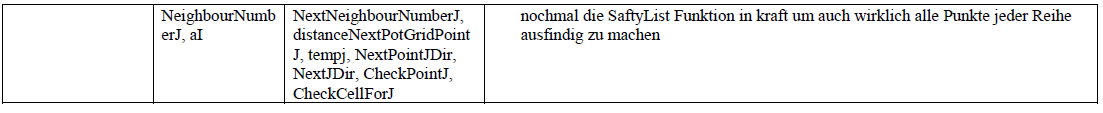
\includegraphics[width=1\linewidth]{images/KD5.png}
	\captionof{figure}{Klassendiagramm}
\end{minipage}\\







